%%%%%%%%%%%%%%%%%%%%% chapter.tex %%%%%%%%%%%%%%%%%%%%%%%%%%%%%%%%%
%
% sample chapter
%
% Use this file as a template for your own input.
%
%%%%%%%%%%%%%%%%%%%%%%%% Springer-Verlag %%%%%%%%%%%%%%%%%%%%%%%%%%
%\motto{Use the template \emph{chapter.tex} to style the various elements of your chapter content.}
\chapter{Mechanistic-empirical models and regression models }
\label{meempi} % Always give a unique label
% use \chaptermark{}
% to alter or adjust the chapter heading in the running head
\chapterauthor{Bryan T. Adey and Nam Lethanh}
\section{General}
\subsection{Manifest and latent processes}
Models are required to predict both the ability to provide a specified level of service (LOS) and the required LOS. The processes that result in changes to either of these can be classified as gradual (manifest) or sudden (latent), depending on how the processes are monitored, the speed with which the infrastructure manager can react and the defined LOS. The classification of a change in LOS as gradual or sudden depends on the state of preparedness and the perception of the infrastructure management owner (IMO). 

A gradual change in the LOS provided is one that happens in a way that there is enough time to execute an intervention so as to ensure that the infrastructure continues to provide an adequate LOS. For example, a gradual change may be the increases in the amount of travel time due to increasingly congested roads, something that may happen at a rate of 2\% per year. 

A sudden change in the LOS provided is one that happens in a way that there is not enough time to execute an intervention so as to ensure that the infrastructure continues to provide an adequate LOS. A sudden change may be a new law that allows the axle loads to increase by 50\%. 

Typical models to be used to predict either the provided or the required LOS due to gradual processes are mechanistic-empirical models, regression models, Markov models, neural network models, and Bayesian networks. 

Typical models to be used to predict with either the provided or the required LOS due to sudden processes are event trees and fault trees.
%
\subsection{Continuous vs. discrete states}
%
Condition of an infrastructure object changes over time. The range of condition in which an object can change before it is referred to as something else is referred to as a ``state''. An adjective or a noun in front of the word ``state'' refers to the factor being used to classify the object. For example, a ``condition state'' is defined based on the physical characteristics of an object, and a ``performance state'' is defined based on the ability of the object to perform, or provide a level of service. 

As states are man-made descriptions of the object there are almost an infinite number of possible ways that states can be defined. How states are defined will affect the illustration of the movement of the object over time through the states. This can be considered in the simplification of the mathematical modeling of the behavior of infrastructure. 
%
\subsection{Deterministic vs. probabilistic models}
Models of the behavior of infrastructure over time can be done using models that are classified as deterministic or probabilistic. Both have advantages and disadvantages.

The use of deterministic models gives the impression that the values of the performance indicators is known with certainty at every time \textit{t}. They give very precise, but perhaps not very accurate predictions.

The use of probabilistic models gives the probability of having each value of the performance indicators at every time \textit{t}. They give less precise predictions than deterministic models but may be more accurate. 
\subsection{Classification of models}
The models that are typically used to make prediction of the future states of infrastructure objects can be classified in different ways. Some examples are given in Table \ref{tbl:31}. The mechanistic-empirical and regression models will be discussed in more detail in the next sections.
\begin{table}
\caption{Types of models for manifest processes}
\begin{tabular}{|l|p{300pt}|}
\hline
Type of model & Definition \\ 
\hline
Analytical & has a closed form solution, i.e. the solution to the equations used to describe changes in a system can be expressed as a mathematical analytic function. \\ 
\hline
Numerical & use some sort of numerical time-stepping procedure to obtain the models behaviour over time \\ 
\hline
Mechanistic & is based on an understanding of the behavior of the elements in a the system, often developed using the laws of physics \\ 
\hline
Empirical & is based on direct observation, measurement and extensive data records, often without understanding the physical processes at work \\ 
\hline
Extrapolation & can be used to estimate a value of a variable outside a known range from values within a known range \\ 
\hline
Interpolation & can be used to estimate a value of a variable within a known range from other values within this range \\ 
\hline
Regression & is developed using regression analysis, which is a statistical approach to predicting the change in the value of a dependent variable based on the changes in the values of an independent variables  \\ 
\hline
Markovian & is stochastic and where the conditional probability distribution of future states of the process (conditional on both past and present values) depends only upon the present state, not on the sequence of events that preceded it \\ 
\hline
\end{tabular}
\label{tbl:31}
\end{table}
\section{Mechanistic-empirical models}
\subsection{Theory}
A mechanistic model is one that is based on an understanding of the behavior of the elements in the system, often developed using the laws of physics. An empirical model is one that is based on direct observation, measurement and extensive data records, often without understanding the physical processes at work. A mechanistic - empirical model is a combination of both.

These types of models are often used to predict the occurrence of very specific conditions, e.g. the amount of chlorides at a specific depth in a concrete beam. Coupled with the probabilistic distributions to represent the values of the variables and parameters in the models, they can be used to estimate the probable specific conditions.

They can also be used to predict a LOS, e.g. the amount of intervention costs in a specified unit of time. Or more specifically, the probability of occurrence of each LOS within each investigated time interval can be estimated using a Monte Carlo simulation or a random sampling algorithm, given the probabilistic distributions of each parameters, and the mechanistic-empirical model.
%
\subsection{Example}
You are an infrastructure manager that would like to predict the evolution of a reinforced concrete bridge slab whose main deterioration process is chloride-induced corrosion of the steel reinforcement over time (More information related to such processes can be found in \cite{Elsener2013} and \cite{Bertolini2013} so that you can plan an intervention before the bridge slab provides an inadequate LOS. You know that the chloride-induced corrosion is composed of two deterioration phases: the first phase is called initiation phase, which covers the entire time from construction to the time the first visual crack appears. In this phase the chloride starts to penetrate into concrete cover, reach the reinforcement with a sufficient concentration to start corrosion and continue until there is enough corrosion to cause cracks to be visible. The second phase of deterioration then starts and includes the continued widening of the cracks in the concrete due to the continued corrosion of the reinforcement. The entire deterioration process can be graphically illustrated in Figure \ref{fig:31}.
\begin{figure}[h]
% \begin{center}
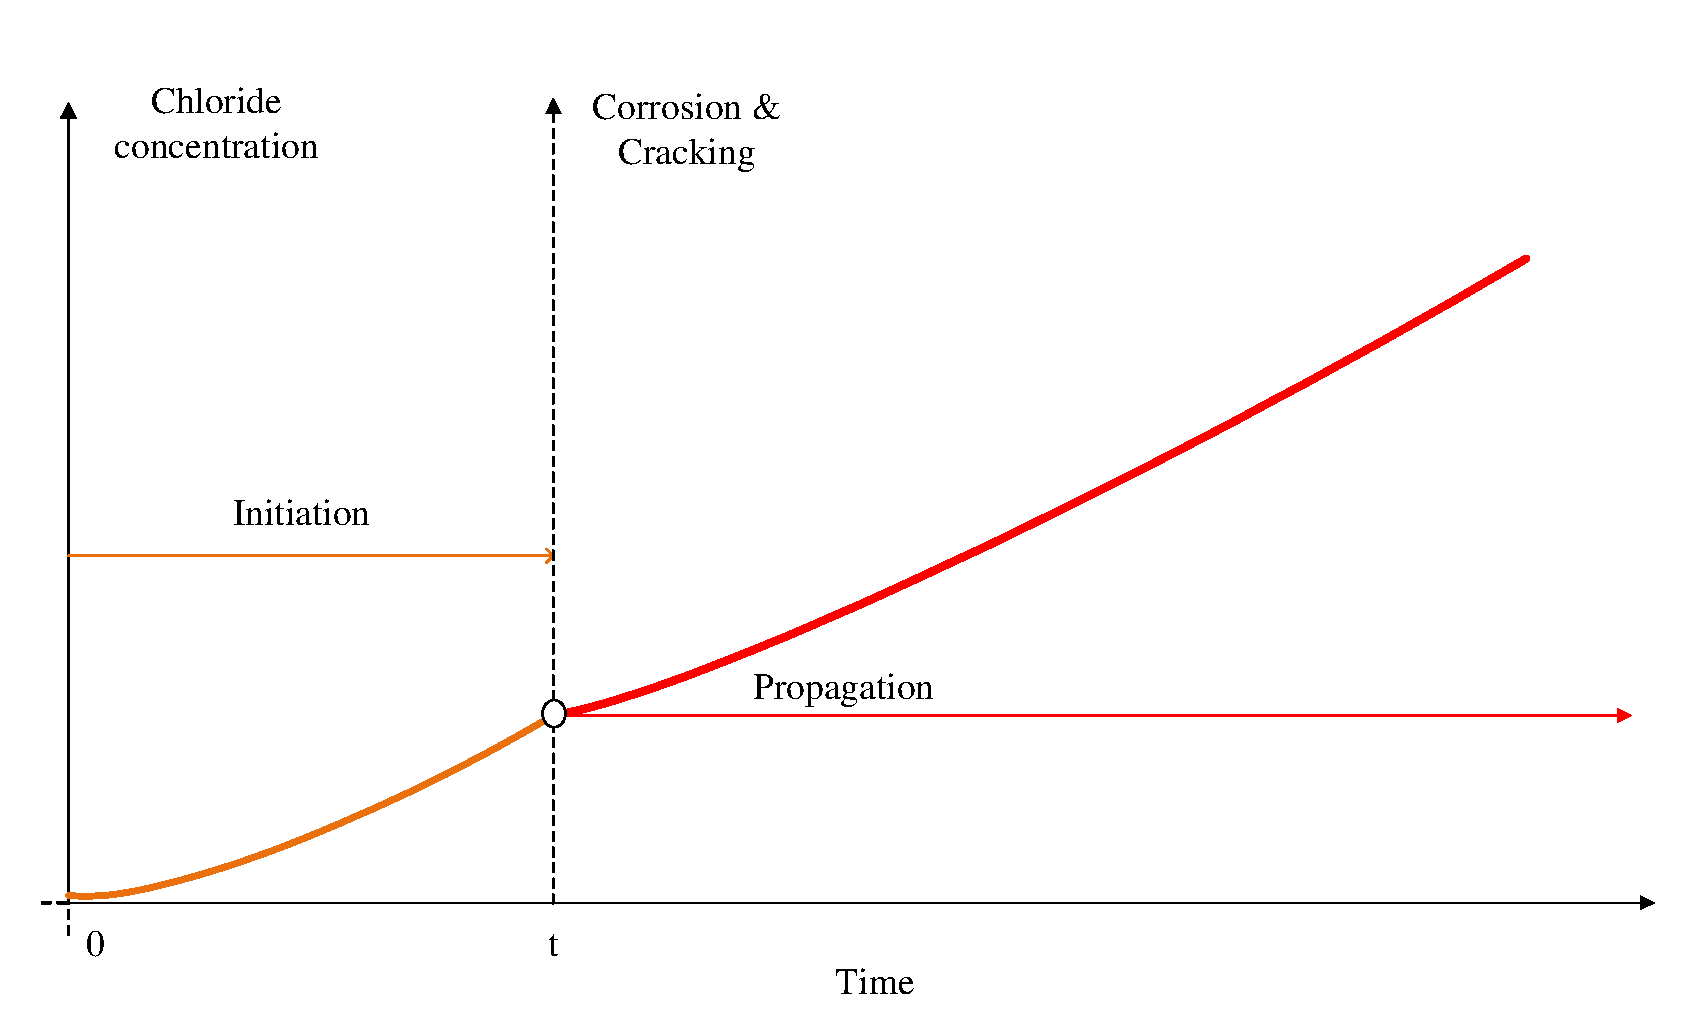
\includegraphics[width=300pt]{fig31.eps}
\caption{Deterioration process of reinforced concrete due to chloride-induced corrosion}\label{fig:31}
% \end{center}
\end{figure}
According to \cite{DuraCrete2000}, chloride penetration into reinforced concrete is a complicated process, which involves inter alia ion diffusion and convection \citep{Bertolini2013}. This complex transport mechanism can be represented by Fick's second law of diffusion.
\begin{eqnarray}
      && \frac{{\partial {C_{cl}}}}{{\partial t}} = {D_{cl}}\frac{{{\partial ^2}{C_{cl}}}}{{\partial x_{cl}^2}} \label{eq31}
\end{eqnarray}
Where:
\begin{adjustwidth}{1cm}{}
\begin{description}
\item[$C_{cl}$:] is the chloride ion concentration at the depth,
\item[$x_{cl}$:] from the surface of concrete after it exposes to chlorides till time \textit{t} (here small notation cl denotes the abbreviation for chloride).  
\item[$D_{cl}$:] is the chloride diffusion coefficient. 
\end{description}
%\end{flushright}
\end{adjustwidth}
The solution for partial differential equation of Eq. \eqref{eq31} gives the following explicit form to calculate the chloride concentration as a function of depth ${x_{cl}}$and time \textit{t}.
\begin{eqnarray}
      && {C_{cl}}({x_{cl}},t) = {C_s}\left( {1 - erf\left( {\frac{{{x_{cl}}}}{{2\sqrt {{D_{cl}}t} }}} \right)} \right) \label{eq32}
\end{eqnarray}
where  $erf\left(  \right)$denotes the error function\footnote{Definition of error function at http://en.wikipedia.org/wiki/Error\_function}. 

The duration for the diffusion process of chloride ion to initiate corrosion, that is time \textit{t} in Eq. \eqref{eq32}, can be estimated by setting the value of ${C_{cl}}$ to be equal to the chloride concentration. In other words, by setting the value of ${C_{cl}}$for each discrete condition state \textit{i}, the time to arrive at that CS can be obtained by solving Eq. \eqref{eq32} with respect to time \textit{t} and a certain depth of concrete cover from the re-bar.

For a bridge slab, value of variables ${C_{cl}}$,${C_s}$, and ${D_{cl}}$in the equation are can be considered as random, each one is associated with its own statistical distribution. Thus, estimation of time to arrive at certain value of chloride concentration is probabilistic in nature.

After the value of chloride concentration reaches a certain limit, corrosion starts on the reinforcing bars and after it reaches another higher limit the cracking process starts. The crack initiation phase is referred to here as the propagation phase and the width of the cracks over time can be determined by using following equations:
\begin{eqnarray}
      && w(t) = {w_0} + \beta  \cdot \left( {P(t) - {P_0}} \right) \label{eq33}
\end{eqnarray}
Where:
\begin{adjustwidth}{1cm}{}
\begin{description}
\item[$w(t)$:] width (mm) of crack over time,
\item[$\beta $:] the parameter that controls the propagation
\item[${w_0}$:] width of crack when it is visible (\textasciitilde{}0.05 mm)
\item[${P_0}$:] the amount of loss of re-bar diameter (mm) when crack width is visible 
\item [$P(t)$:] the amount of loss of re-bar diameter (mm) at \textit{t}
\end{description}
%\end{flushright}
\end{adjustwidth}

The reinforcement loss function can be represented as:
%
\begin{eqnarray}
      && P(t) = \int\limits_0^t {{V_{corr}} \cdot \alpha  \cdot wet \cdot tdt}  \label{eq34}
\end{eqnarray}
Where:
\begin{adjustwidth}{1cm}{}
\begin{description}
\item[${V_{corr}}$:] corrosion rate coefficient (mm/year)
\item[$wet$:] wet period in a year (equal to the ratio between total numbers of rainy day and 365 days)
\item[$\alpha $:] pitting factor that takes non-uniform corrosion of the re-bars into consideration
\end{description}
%\end{flushright}
\end{adjustwidth}

Based on field tests and experiments, statistical values of models coefficients and parameters are given in Table \ref{tbl:32}
% 
\begin{table}
\caption{Values of models parameters and coefficients}
\begin{tabular}{|l|l|l|l|l|l|}
\hline
\multicolumn{1}{|c|}{Parameters/ Coefficients} & \multicolumn{1}{c|}{Units} & Mean ($\mu$) & Standard deviation ($\sigma$) & Distribution & Reference equations \\ 
\hline
\multicolumn{1}{|c|}{$C_s$} & \multicolumn{1}{c|}{$wt.-\%Cl-/binder$} & \multicolumn{1}{c|}{2.565} & \multicolumn{1}{c|}{0.405} & \multicolumn{1}{c|}{Normal} & \multicolumn{1}{c|}{Eq. \eqref{eq32}} \\ 
\hline
\multicolumn{1}{|c|}{$x_{cl}$} & \multicolumn{1}{c|}{mm} & \multicolumn{1}{c|}{20} & \multicolumn{1}{c|}{NA} & \multicolumn{1}{c|}{NA} & \multicolumn{1}{c|}{Eq. \eqref{eq32}} \\ 
\hline
\multicolumn{1}{|c|}{$D_{cl}$} & \multicolumn{1}{c|}{NA} & \multicolumn{1}{c|}{100} & \multicolumn{1}{c|}{0.5} & \multicolumn{1}{c|}{Normal} & \multicolumn{1}{c|}{Eq. \eqref{eq32}} \\ 
\hline
\multicolumn{1}{|c|}{$w_0$} & \multicolumn{1}{c|}{mm} & \multicolumn{1}{c|}{0.05} & \multicolumn{1}{c|}{0.005} & \multicolumn{1}{c|}{Normal} & \multicolumn{1}{c|}{Eq. \eqref{eq33}} \\ 
\hline
\multicolumn{1}{|c|}{$P_0$} & \multicolumn{1}{c|}{mm} & \multicolumn{1}{c|}{5} & \multicolumn{1}{c|}{0.5} & \multicolumn{1}{c|}{Normal} & \multicolumn{1}{c|}{Eq. \eqref{eq33}} \\ 
\hline
\multicolumn{1}{|c|}{$\beta$} & \multicolumn{1}{c|}{NA} & \multicolumn{1}{c|}{0.001} & \multicolumn{1}{c|}{0.001} & \multicolumn{1}{c|}{Normal} & \multicolumn{1}{c|}{Eq. \eqref{eq33}} \\ 
\hline
\multicolumn{1}{|c|}{$V_{corr}$} & \multicolumn{1}{c|}{} & \multicolumn{1}{c|}{0.012} & \multicolumn{1}{c|}{0.006} & \multicolumn{1}{c|}{Normal} & \multicolumn{1}{c|}{Eq. \eqref{eq34}} \\ 
\hline
\multicolumn{1}{|c|}{$wet$} & \multicolumn{1}{c|}{year} & \multicolumn{1}{c|}{1} & \multicolumn{1}{c|}{0.25} & \multicolumn{1}{c|}{Normal} & \multicolumn{1}{c|}{Eq. \eqref{eq34}} \\ 
\hline
\multicolumn{1}{|c|}{$\alpha$} & \multicolumn{1}{c|}{NA} & \multicolumn{1}{c|}{14} & \multicolumn{1}{c|}{4.04} & \multicolumn{1}{c|}{Normal} & \multicolumn{1}{c|}{Eq. \eqref{eq34}} \\ 
\hline
\end{tabular}
\label{tbl:32}
\end{table}

\subsubsection{Question}
If you know that the chloride concentration ${C_{crit}}$ which starts the propagation phase is ${C_{cl}} = {C_{crit}} = 0.48$, and you consider that once a crack width is 0.5 mm, that an intervention is required to ensure that an adequate LOS is provided, when do you need to plan an intervention to ensure that an adequate LOS is provided? 

Hint: Construct a probabilistic deterioration model with discrete condition states for the entire chloride induced corrosion process of the bridge slab.
\subsubsection{Answer}
\paragraph{Condition states}
Since the deterioration process of chloride induced corrosion is a continuous process with two distinct phases, it is useful to define ranges of condition states for each phase in order to construct the probabilistic deterioration model with discrete condition states. This is illustrated in Figure \ref{fig:32}, when 5 condition states are used. Two are attributed to the initiation phase and two to the propagation phase.
\begin{figure}[h]
% \begin{center}
\includegraphics[width=300pt]{fig32.eps}
\caption{Deterioration process with discrete condition states}\label{fig:32}
% \end{center}
\end{figure}
In Figure \ref{fig:32}, five discrete condition states are used to illustrate the process. Their definitions are explained in Table \ref{tbl:33}.

\begin{table}
%	\centering
	\caption{Definition of condition states} \label{tbl:33}
		\begin{tabular}{|l|l|p{3.5cm}|p{5.5cm}|l|}
\hline
\multicolumn{1}{|c|}{Phase} & \multicolumn{1}{c|}{CS} & \multicolumn{1}{c|}{Description} & \multicolumn{1}{c|}{Indicator} & \multicolumn{1}{c|}{Criteria} \\ 
\hline
\multicolumn{1}{|c|}{1} & \multicolumn{1}{c|}{1} & New/partial new & Amount of chlorides in & \multicolumn{1}{c|}{$0 < C_{cl}\le 0.24$} \\ 
\cline{2-3}\cline{5-5}
\multicolumn{1}{|c|}{} & \multicolumn{1}{c|}{2} & Concrete contaminated & the concrete at reinforcing bar level $C_{cl}$ & \multicolumn{1}{c|}{$0.24 < C_{cl}\le 0.48$} \\ 
\hline
\multicolumn{1}{|c|}{2} & \multicolumn{1}{c|}{3} & Corrosion has initiated, no visible cracking has occurred & \multicolumn{1}{c|}{} & \multicolumn{1}{c|}{$C_{cl}> 0.48, w\le 0.25$} \\ 
\cline{2-3}\cline{5-5}
\multicolumn{1}{|c|}{} & \multicolumn{1}{c|}{4} & Visible cracking has occurred & Width of crack ($w$) & \multicolumn{1}{c|}{$0.25 < w \le 0.5$} \\ 
\cline{2-3}\cline{5-5}
\multicolumn{1}{|c|}{} & \multicolumn{1}{c|}{5} & Visible cracking has occurred and cover has spalled off & \multicolumn{1}{c|}{} & \multicolumn{1}{c|}{$ w > 0.5$} \\ 
\hline
\end{tabular}
\end{table}

\paragraph{Deterioration: Chloride concentration}

Using Eq. \eqref{eq32}, the concentration of chlorides at any time \textit{t} can be deterministically estimated given the mean values of the parameters of the model. These are, however, probabilistic in nature, thus, an explicit and straightforward arithmetic calculation is not always desirable. At any time in the future, for example, the value of ${C_{cl}}$ can be represented by using the mean and standard deviation. This concept is illustrated in Figure \ref{fig:33} for a normal distribution, where the mean value $\mu$ and standard deviation $\sigma$ are 0.3 and 0.08, respectively

\begin{figure}[h]
% \begin{center}
\includegraphics[width=300pt]{fig33.eps}
\caption{Probability of condition state CS 1-initiation phase.}\label{fig:33}
% \end{center}
\end{figure}
 
In order to determine when an intervention is required to ensure that an adequate LOS is provided, the probability of being in each condition state over time needs to be calculated.

Let assume that it is time \textit{t} now, and the probability of the bridge slab being in CS 1 will be equivalent to the probability that its continuous value falls between 0 and 0.24. The equation used to estimate the red area is.

In order to determine when an intervention is required to ensure that an adequate LOS is provided, the probability of being in each condition state over time needs to be calculated. 

Let assume that it is time t now, and the probability of the bridge slab being in $CS1$ will be equivalent to the probability that its continuous value falls between 0 and 0.24. The equation used to estimate the red area is.
\begin{eqnarray}
      && P_1 =P_1^{cl} = Prob[CS=1]=Prob[0 \leq C_{cl} \leq 0.24] = \int_0^{0.24}f(x) \cdot dx = 0.227 \label{stateprobcs1}
\end{eqnarray}
where $f(x)$ is density function of the normal distribution. 
\begin{eqnarray}
      && f(x)= \frac{1}{\sigma \sqrt{2\pi}}\cdot e^{-\frac{(x-\mu)^2}{2\sigma^2}}\label{densitynormaldistribu}
\end{eqnarray}
Similarly, the probability that the bridge element is in $CS2$ is given by:
\begin{eqnarray}
      && P_2 = P_2^{cl} = Prob[CS=2]=Prob[0.24 \leq C_{cl} \leq 0.48] \nonumber \\
      && = \int_{0.24}^{0.48}f(x) \cdot dx = 0.761 \label{stateprobcs2}
\end{eqnarray}
The probability that the bridge slab is in $CS3$ is in a condition state greater than CS2 is then given by:
\begin{eqnarray}
      && P_{>2} = P_{>2}^{cl} = 1-Prob[CS=2]-Prob[CS=2]=1-0.227-0.761=0.012\label{stateprobcs345}
\end{eqnarray}
%
\begin{figure}[h!]
% \centering
\includegraphics[width=300pt]{fig34.eps} 
\caption{Probability of condition state CS-2-initiation phase.} 
\label{fig:34}
\end{figure}
%
\paragraph{Deterioration: Corrosion propagation}

If it is assumed that the crack width can be modeled using a normal distribution with $\left[ {\mu  = 0.22,\sigma  = 0.03} \right]$ at time \textit{t} (the same time that is used to compute the state probability of the initiation phase), then the probability of being in condition state 3 is given by: 

\begin{figure}[h]
% \begin{center}
\includegraphics[width=300pt]{fig35.eps}
\caption{Probability of condition state CS 3-propagation phase.}
% \end{center}
\end{figure}

\begin{eqnarray}
      && P_3 = P_3^{cr} = Prob[CS=3]=Prob[w\leq0.25]\cdot Prob[C_{cl}>0.48] \nonumber \\
      && = 0.841 \cdot 0.012 = 0.010092\label{eq35}
\end{eqnarray}

Eq. \eqref{eq35} shows a joint probability of the event that chloride concentration level has reached more than its critical level 0.48 and corrosion has progressed to a point where at least one crack of 0.05 mm has opened up. The width of crack is, however, less than 0.25 mm.

Similarly, following state transition probabilities are obtained

\begin{eqnarray}
      && P_4 = P_4^{cr} = Prob[CS=4]=Prob[0.25 <w\leq0.5]\cdot Prob[C_{cl}>0.48] \nonumber \\
      && = 0.159 \cdot 0.012 = 0.001908\label{stateprobcs4} \\
      && P_5 = P_5^{cr} = Prob[CS=5]=Prob[w\geq 0.5]\cdot Prob[C_{cl}>0.48] = 0 \cdot 0.012 = 0 \label{stateprobcs5}
\end{eqnarray}

The above steps of calculation are used for a specific case when the condition state is defined in Table \ref{tbl:33}. For a general case that mathematically describes the relationship and for sake of programing, following generic formulation is used.

%
\begin{eqnarray}
&& {P_k} = \left\{ {\begin{array}{*{10}{c}}
{P_i^{cl} = \int\limits_a^b {f(x)dx} \hspace{0.2cm}i = (1,...,I){\rm{  }}}\\
{P_I^{cl} \cdot P_j^{cr} \hspace{1cm}   where \hspace{1cm} P_j^{cr} = \int\limits_c^d {g(x)dx} \hspace{1cm}j = (1,...,J)}
\end{array}{\rm{    }}} \right. \label{eq36}
\end{eqnarray}

Where:%k = (1,...,\left[ {I + J - 1} \right])
\begin{adjustwidth}{1cm}{}
\begin{description}
\item[$P_i^{cl}$:] is state probability of CS $i$ of the initiation phase with total number CS of $I$
\item[$P_j^{cl}$:] is state probability of CS $j$ of the propagation phase with total number CS of $J$
\item[$f(x)$ and $g(x)$:] are density function of the normal distribution for the initiation phase and propagation phase, respectively.
\end{description}
%\end{flushright}
\end{adjustwidth}
\paragraph{State distribution as proportional data}
Once the mechanistic-empirical equation, and the probabilistic distributions of each parameter to be used are known than the probable value of both chloride concentration and crack width can be generated by running many simulations, e.g. $20’000$. Once enough points are generated at the point of time to be investigated, either the probabilistic distribution that best fits these points can be determined and from this distribution the probability of the bridge slab being in a specific condition state can be estimated, or the probability of the bridge being in each condition state can be estimated directly from the number of data points, e.g. $10’000/20’000$ are in the specified range. 

In previous steps of calculation, the example is shown only for a specific time $t$ given the mean $\mu$ and the standard deviation $\sigma$ for each process. However, these values have to be estimated at each time step given the probabilistic distribution of models parameters. Results of estimation are the state probabilities over a pre-defined number of years. This pool of state probabilities is proportional data and state probabilities of the bridge in previous year is not related to the following year.

\paragraph{Deterioration prediction}

Once the mechanistic-empirical equation, and the probabilistic distributions of each parameter to be used are known than the probable value of both chloride concentration and crack width can be generated by running many simulations, e.g. 20'000. Once enough points are generated at the point of time to be investigated, either the probabilistic distribution that best fits these points can be determined and from this distribution the probability of the bridge slab being in a specific condition state can be estimated, or the probability of the bridge being in each condition state can be estimated directly from the number of data points, e.g. 10'000 / 20'000 are in the specified range. 

In previous steps of calculation, the example is shown only for a specific time \textit{t} given the mean $\mu$ and the standard deviation $\sigma$ for each process. However, these values have to be estimated at each time step given the probabilistic distribution of models parameters (Table \ref{tbl:32}).

Results of the estimation are the state probability over a pre-defined number of years. In this example, calculation is done for 60 years. At each year, the probabilistic value of chloride concentration ${C_{cl}}$ and the width of crack $X$ are re-computed using a pool of 20'000 samples that were randomly generated using Monte Carlo simulation. Then, the state probability that the bridge slab arrives at each discrete CS was computed for every year. These are shown in graphically in Figure \ref{fig:36}. 

\begin{figure}[h]
% \begin{center}
\includegraphics[width=324pt]{fig36.eps}
\caption{Condition state distribution over 60 years}\label{fig:36}
% \end{center}
\end{figure}
 
\paragraph{Results}

As can be seen from Figure \ref{fig:36}, in the first 7 years after the construction of the bridge slab, the chloride concentration is not expected to reach a value of 0.25. In other words, the bridge slab is expected to remain in CS 1. Then, the probability of the bridge slab being in CS 1 decreases, in the mean-time, of course, the probability that the bridge slab is in CS 2 increases. After 10 years, there is almost a 50\% chance that the bridge slab will be in CS 2.

Between the 7$^{th}$ and 10$^{th}$ years, there is a non-zero probability that the critical chloride concentration has been reached (0.48), i.e. the propagation phase has started. This explains the appearance of CS 3, CS 4 and CS 5 in the chart.

After 20 years, there is a high probability that the critical chloride concentration has been reached and the propagation phase has started. There is also approximately a 40\% chance that the surface of the slab will have at least one crack with a width between 0.00 mm and 0.25 mm. More or less the same chance that the crack width will be between 0.25 mm and 0.5 mm. There is, however, also a 20\% chance that the crack width will be greater than 0.5 mm, and that an intervention will have to be executed to ensure that an adequate LOS is provided.

So, since I know that the chloride concentration ${C_{crit}}$ that starts the propagation phase is ${C_{cl}} = {C_{crit}} = 0.48$, and if I consider that once a crack width is 0.5 mm that an intervention is required to ensure that an adequate LOS is provided, I will plan an intervention in year 15, when the probability of being in CS5 is still, according to my calculations is under 0.01 (Table \ref{tbl:34}). 
\begin{table}
%	\centering
	\caption{Evolution of state probability over 30 years} \label{tbl:34}
\begin{tabular}{|l|l|l|l|l|l|}
\hline
\multicolumn{1}{|m{1.5cm}|}{\centering year} & \multicolumn{5}{c|}{Condition states} \\ 
\cline{2-6}
\multicolumn{1}{|c|}{} & \multicolumn{1}{m{1.5cm}|}{\centering 1} & \multicolumn{1}{m{1.5cm}|}{\centering 2} & \multicolumn{1}{m{1.5cm}|}{\centering 3} & \multicolumn{1}{m{1.5cm}|}{\centering 4} & \multicolumn{1}{m{1.5cm}|}{\centering 5} \\ 
\hline
\multicolumn{1}{|c|}{1} & \multicolumn{1}{c|}{1} & \multicolumn{1}{c|}{0} & \multicolumn{1}{c|}{0} & \multicolumn{1}{c|}{0} & \multicolumn{1}{c|}{0} \\ 
\hline
\multicolumn{1}{|c|}{2} & \multicolumn{1}{c|}{1} & \multicolumn{1}{c|}{0} & \multicolumn{1}{c|}{0} & \multicolumn{1}{c|}{0} & \multicolumn{1}{c|}{0} \\ 
\hline
\multicolumn{1}{|c|}{3} & \multicolumn{1}{c|}{1} & \multicolumn{1}{c|}{0} & \multicolumn{1}{c|}{0} & \multicolumn{1}{c|}{0} & \multicolumn{1}{c|}{0} \\ 
\hline
\multicolumn{1}{|c|}{4} & \multicolumn{1}{c|}{1} & \multicolumn{1}{c|}{0} & \multicolumn{1}{c|}{0} & \multicolumn{1}{c|}{0} & \multicolumn{1}{c|}{0} \\ 
\hline
\multicolumn{1}{|c|}{5} & \multicolumn{1}{c|}{1} & \multicolumn{1}{c|}{0} & \multicolumn{1}{c|}{0} & \multicolumn{1}{c|}{0} & \multicolumn{1}{c|}{0} \\ 
\hline
\multicolumn{1}{|c|}{6} & \multicolumn{1}{c|}{1} & \multicolumn{1}{c|}{0} & \multicolumn{1}{c|}{0} & \multicolumn{1}{c|}{0} & \multicolumn{1}{c|}{0} \\ 
\hline
\multicolumn{1}{|c|}{7} & \multicolumn{1}{c|}{0.9174} & \multicolumn{1}{c|}{0.0826} & \multicolumn{1}{c|}{0} & \multicolumn{1}{c|}{0} & \multicolumn{1}{c|}{0} \\ 
\hline
\multicolumn{1}{|c|}{8} & \multicolumn{1}{c|}{0.5520} & \multicolumn{1}{c|}{0.3907} & \multicolumn{1}{c|}{0.0574} & \multicolumn{1}{c|}{0} & \multicolumn{1}{c|}{0} \\ 
\hline
\multicolumn{1}{|c|}{9} & \multicolumn{1}{c|}{0.2977} & \multicolumn{1}{c|}{0.3571} & \multicolumn{1}{c|}{0.3452} & \multicolumn{1}{c|}{0} & \multicolumn{1}{c|}{0} \\ 
\hline
\multicolumn{1}{|c|}{10} & \multicolumn{1}{c|}{0.1718} & \multicolumn{1}{c|}{0.2123} & \multicolumn{1}{c|}{0.6149} & \multicolumn{1}{c|}{0.001} & \multicolumn{1}{c|}{0} \\ 
\hline
\multicolumn{1}{|c|}{11} & \multicolumn{1}{c|}{0.1065} & \multicolumn{1}{c|}{0.1181} & \multicolumn{1}{c|}{0.7640} & \multicolumn{1}{c|}{0.0114} & \multicolumn{1}{c|}{0} \\ 
\hline
\multicolumn{1}{|c|}{12} & \multicolumn{1}{c|}{0.0693} & \multicolumn{1}{c|}{0.0672} & \multicolumn{1}{c|}{0.8153} & \multicolumn{1}{c|}{0.0482} & \multicolumn{1}{c|}{0} \\ 
\hline
\multicolumn{1}{|c|}{13} & \multicolumn{1}{c|}{0.0466} & \multicolumn{1}{c|}{0.0396} & \multicolumn{1}{c|}{0.7965} & \multicolumn{1}{c|}{0.1173} & \multicolumn{1}{c|}{0.0001} \\ 
\hline
\multicolumn{1}{|c|}{14} & \multicolumn{1}{c|}{0.0319} & \multicolumn{1}{c|}{0.0242} & \multicolumn{1}{c|}{0.7360} & \multicolumn{1}{c|}{0.2069} & \multicolumn{1}{c|}{0.0011} \\ 
\hline
\multicolumn{1}{|c|}{15} & \multicolumn{1}{c|}{0.0221} & \multicolumn{1}{c|}{0.0151} & \multicolumn{1}{c|}{0.6584} & \multicolumn{1}{c|}{0.2977} & \multicolumn{1}{c|}{0.0068} \\ 
\hline
\multicolumn{1}{|c|}{16} & \multicolumn{1}{c|}{0.0154} & \multicolumn{1}{c|}{0.0097} & \multicolumn{1}{c|}{0.5795} & \multicolumn{1}{c|}{0.3720} & \multicolumn{1}{c|}{0.0234} \\ 
\hline
\multicolumn{1}{|c|}{17} & \multicolumn{1}{c|}{0.0107} & \multicolumn{1}{c|}{0.0063} & \multicolumn{1}{c|}{0.5073} & \multicolumn{1}{c|}{0.4195} & \multicolumn{1}{c|}{0.0561} \\ 
\hline
\multicolumn{1}{|c|}{18} & \multicolumn{1}{c|}{0.0075} & \multicolumn{1}{c|}{0.0041} & \multicolumn{1}{c|}{0.4447} & \multicolumn{1}{c|}{0.4387} & \multicolumn{1}{c|}{0.1050} \\ 
\hline
\multicolumn{1}{|c|}{19} & \multicolumn{1}{c|}{0.0052} & \multicolumn{1}{c|}{0.0027} & \multicolumn{1}{c|}{0.3918} & \multicolumn{1}{c|}{0.4344} & \multicolumn{1}{c|}{0.1659} \\ 
\hline
\multicolumn{1}{|c|}{20} & \multicolumn{1}{c|}{0.0036} & \multicolumn{1}{c|}{0.0018} & \multicolumn{1}{c|}{0.3477} & \multicolumn{1}{c|}{0.4139} & \multicolumn{1}{c|}{0.2330} \\ 
\hline
\multicolumn{1}{|c|}{21} & \multicolumn{1}{c|}{0.0025} & \multicolumn{1}{c|}{0.0012} & \multicolumn{1}{c|}{0.3110} & \multicolumn{1}{c|}{0.3842} & \multicolumn{1}{c|}{0.3011} \\ 
\hline
\multicolumn{1}{|c|}{22} & \multicolumn{1}{c|}{0.0017} & \multicolumn{1}{c|}{0.0008} & \multicolumn{1}{c|}{0.2805} & \multicolumn{1}{c|}{0.3506} & \multicolumn{1}{c|}{0.3664} \\ 
\hline
\multicolumn{1}{|c|}{23} & \multicolumn{1}{c|}{0.0012} & \multicolumn{1}{c|}{0.0005} & \multicolumn{1}{c|}{0.2551} & \multicolumn{1}{c|}{0.3164} & \multicolumn{1}{c|}{0.4268} \\ 
\hline
\multicolumn{1}{|c|}{24} & \multicolumn{1}{c|}{0.0008} & \multicolumn{1}{c|}{0.0004} & \multicolumn{1}{c|}{0.2337} & \multicolumn{1}{c|}{0.2839} & \multicolumn{1}{c|}{0.4812} \\ 
\hline
\multicolumn{1}{|c|}{25} & \multicolumn{1}{c|}{0.0006} & \multicolumn{1}{c|}{0.0002} & \multicolumn{1}{c|}{0.2157} & \multicolumn{1}{c|}{0.2539} & \multicolumn{1}{c|}{0.5296} \\ 
\hline
\multicolumn{1}{|c|}{26} & \multicolumn{1}{c|}{0.0004} & \multicolumn{1}{c|}{0.0002} & \multicolumn{1}{c|}{0.2005} & \multicolumn{1}{c|}{0.2269} & \multicolumn{1}{c|}{0.5721} \\ 
\hline
\multicolumn{1}{|c|}{27} & \multicolumn{1}{c|}{0.0003} & \multicolumn{1}{c|}{0.0001} & \multicolumn{1}{c|}{0.1874} & \multicolumn{1}{c|}{0.2030} & \multicolumn{1}{c|}{0.6093} \\ 
\hline
\multicolumn{1}{|c|}{28} & \multicolumn{1}{c|}{0.0002} & \multicolumn{1}{c|}{0.0001} & \multicolumn{1}{c|}{0.1762} & \multicolumn{1}{c|}{0.1819} & \multicolumn{1}{c|}{0.6417} \\ 
\hline
\multicolumn{1}{|c|}{29} & \multicolumn{1}{c|}{0.0001} & \multicolumn{1}{c|}{0} & \multicolumn{1}{c|}{0.1664} & \multicolumn{1}{c|}{0.1634} & \multicolumn{1}{c|}{0.6700} \\ 
\hline
\multicolumn{1}{|c|}{30} & \multicolumn{1}{c|}{0.0001} & \multicolumn{1}{c|}{0} & \multicolumn{1}{c|}{0.1580} & \multicolumn{1}{c|}{0.1472} & \multicolumn{1}{c|}{0.6947} \\ 
\hline
\end{tabular}
\end{table}
As I know, however, that CS5 does not necessarily mean that an inadequate LOS is provided, I can also treat it as a warning that an inadequate LOS is coming if I don't do anything, but that I have a bit of time before this will happen. In this case, I may plan the intervention to be in year 20, when the probability of being in CS5 is 0.233. If I decide to wait until there is 50\% of being in CS5 than I will plan the intervention for either year 24 or 25. Whether or not this is a good decision depends on the probability of an inadequate LOS occurring once the slab reaches CS5 and the consequences if the adequate LOS happens, i.e. the risk associated with being in CS5.

The steps of numerical calculation can be tracked by reading the R script for this example provided at the Appendix \ref{mepi1}.
%
\section{Regression models} \label{regressionmodel}
\subsection{Theory}
Regression models represent empirical relationships between multiple parameters and are developed using regression analysis. They are used to predict the change in the value of a dependent variable based on the changes in the values of independent variables. Each variable is described in terms of its mean and variance. The simplest form is a linear regression model as shown in equation \ref{eq37}. Other forms are possible.

\begin{eqnarray}
 && {Y_i} = \alpha  + \beta  \cdot {X_i} + {\varepsilon _i} \label{eq37}
\end{eqnarray}
Where:
\begin{adjustwidth}{1cm}{}
\begin{description}
\item[${Y_i}$:] is the dependent variable or output (e.g. state probability of \textit{CS i}) that is observable
\item[${X_i}$:] is the characteristic or explanatory variable that is also observable (e.g. time, traffic volume, ambient temperature).
\item[$\alpha ,\beta $:] are parameters that need to be estimated.
\item[$\varepsilon $:] is the prediction error that can be assumed to follow a certain distribution (e.g. normal or log-normal distributions)
\end{description}
%\end{flushright}
\end{adjustwidth}

The mean or expected value of $Y_i$ for each value of input $X_i$ is
\begin{eqnarray}
 && E{Y_i} = \hat{\alpha}  + \hat{\beta}  \cdot {X_i} + {\varepsilon _i} \label{eq38}
\end{eqnarray}
The overhead mark ${\rm{\hat{\hspace{1mm}}}}$ indicates the expected values.

The purpose of performing a regression analysis is to predict the expected values of the regression parameters $\hat \alpha ,\hat \beta $ that minimize following objective function.
\begin{eqnarray}
 && s = {\sum\limits_{i = 1}^N {\left[ {{Y_i} - {{\hat Y}_i}} \right]} ^2} = {\sum\limits_{i = 1}^N {\left[ {{Y_i} - \hat \alpha  - \hat \beta  \cdot {X_i}} \right]} ^2} \label{eq39}
\end{eqnarray}

In words, the objective of Eq. \eqref{eq39} is to minimize the sum of the prediction errors. Here \textit{N} is the total of data points. 

In order to obtain the values of the regression parameters, one way of analytically solving Eq. \eqref{eq39} with respect to two variables $\hat \alpha ,\hat \beta $ (hereafter refer as a vector set $\hat \theta $). This can be done by taking the first derivative of Eq. \eqref{eq39} and set it to be equal to 0, and then solve for $\hat \theta $.
\begin{eqnarray}
 && \frac{{\partial s}}{{\partial \hat \theta }} = 0 \label{eq310}
\end{eqnarray}
For the value of $\hat \alpha $
\begin{manyeqns}
 && \frac{{\partial s}}{{\partial \hat \alpha }} = 0 \label{eq311} \\
 && \Leftrightarrow \frac{{{{\bar Y}^2} - 2 \cdot \bar Y(\hat \alpha  + \hat \beta  \cdot \bar X) + {{(\hat \alpha  + \hat \beta  \cdot \bar X)}^2}}}{{\partial \hat \alpha }} = 0\\
 && \Leftrightarrow  - 2 \cdot \bar Y + 2 \cdot \hat \alpha  + 2 \cdot \hat \beta  \cdot \bar X = 0\\
 && \Leftrightarrow \hat \alpha  = \bar Y - \hat \beta  \cdot \bar X
\end{manyeqns}
%
Here, the bar ${\rm{\bar{\hspace{1mm}}  }}$ indicates the value of $\frac{{\sum\limits_{i = 1}^N {{X_i}} }}{N}$ and $\frac{{\sum\limits_{i = 1}^N {{Y_i}} }}{N}$, which are the mean values.

Similarly, for the value of $\hat \beta $
\begin{manyeqns}
  && \frac{{\partial s}}{{\partial \hat \beta }} = 0\\
 && \Leftrightarrow \frac{{{{\bar Y}^2} - 2 \cdot \bar Y(\hat \alpha  + \hat \beta  \cdot \bar X) + {{(\hat \alpha  + \hat \beta  \cdot \bar X)}^2}}}{{\partial \hat \beta }} = 0\\
 && \Leftrightarrow \beta  \cdot \sum\limits_{i = 1}^N {X_i^2}  - \sum\limits_{i = 1}^N {{X_i} \cdot {Y_i}}  + \alpha \sum\limits_{i = 1}^N {{X_i}}  = 0\\
 && \Leftrightarrow \frac{{\sum\limits_{i = 1}^N {{X_i} \cdot {Y_i}}  - n \cdot \bar X \cdot \bar Y}}{{\sum\limits_{i = 1}^N {X_i^2 - n \cdot \bar X} }} = \frac{{\sum\limits_{i = 1}^N {({X_i} - \bar X) \cdot ({Y_i} - \bar Y)} }}{{\sum\limits_{i = 1}^N {{{({X_i} - \bar X)}^2}} }}
\end{manyeqns}
Following figure graphically represents the regression equation and the calculation.

\begin{figure}[h]
% \begin{center}
\includegraphics[width=300pt]{fig37.eps}
\caption{Deriving linear regression coefficients}
% \end{center}
\end{figure}

The goodness of fit of the regression line can be measured by the coefficient ${R^2}$, which measures the proportion of total variation about the mean $\bar Y$, which is explained by regression:
\begin{eqnarray}
 && {R^2} = \frac{{\sum\limits_{i = 1}^N {{{({{\hat Y}_i} - \bar Y)}^2}} }}{{\sum\limits_{i = 1}^N {{{({Y_i} - \bar Y)}^2}} }} = \frac{{{\beta ^2} \cdot \sum\limits_{i = 1}^N {{{({X_i} - \bar X)}^2}} }}{{\sum\limits_{i = 1}^N {{{({{\hat Y}_i} - \bar Y)}^2}} }} \label{eq321}
\end{eqnarray}
The prediction errors can be followed an independent type of distribution. In many practical situation, normal distribution is often used. In case of normal distribution $N(\mu ,\sigma )$, its mean and standard deviation are defined as:
\begin{eqnarray}
 && {\mu _\varepsilon } = {Y_i} - {\hat Y_i} \label{eq322}\\
 && {\sigma _\varepsilon } = \sqrt {\frac{{\sum\limits_{i = 1}^N {{{({Y_i} - {Y_i})}^2}} }}{{N - k - 1}}}
\end{eqnarray}
Where \textit{k} is number of independent variable, which is equal to 1 in this example (as there is only one input X).

The above example is for the case of simple linear regression with only one independent variable. In many practical situations, linear regression models can be built for multiple variables, which often takes following form.
\begin{eqnarray}
 && Y = \sum\limits_{i = 0}^N {\beta _{}^k}  \cdot X_i^k \label{eq3223}
\end{eqnarray}
Where $k = 1,...,K$ is a vector set of numbers of independent variables. 
\subsection{Example}
Assuming that you have many reinforced concrete slabs, as the one discussed in section 2.2 and have measured chloride concentrations and crack widths over the years, you may have the plots shown in Figure \ref{fig:38} and Figure \ref{fig:39}\footnote{Data used for this example is selected from the pool of randomly generated total data used in the previous example, taking into consideration of the mean and standard deviation at each time t.}. (This data will be distributed in a .csv file in addition to this text).
\begin{figure}[h]
%\begin{center}
\includegraphics[width=300pt]{fig38.eps}
\caption{Measured chloride concentrations in similar deck slabs over time}\label{fig:38}
%\end{center}
\end{figure}
\begin{figure}[h]
%\begin{center}
\includegraphics[width=300pt]{fig39.eps}
\caption{Measured crack widths in similar deck slabs over time}\label{fig:39}
%\end{center}
\end{figure}
\subsubsection{Question}
If you know that the chloride concentration ${C_{crit}}$ which starts the propagation phase is ${C_{cl}} = {C_{crit}} = 0.48$, as in the previous example, and you consider that the once a crack width of 0.5 mm is reached, that an intervention is required to ensure that an adequate LOS is provided, when do you need to plan an intervention to ensure that an adequate LOS is provided? (Use linear regression analysis with the values of chloride concentration and crack width provided, estimate the functional form of deterioration).
\subsubsection{Answer}
As deterioration of the bridge slab is seen as happening in two different phases, separate models are developed using regression analysis for both phases; one for the initiation phase with chloride concentration and other for the propagation phase with the development of crack.
\paragraph{Condition states}
The condition states are defined exactly as in Table \ref{tbl:33}.
\paragraph{Deterioration: Chloride concentration} \label{chrloride}
The form of regression equation for chloride concentration, when it is assumed to be linear is:
\begin{eqnarray}
 && Y_i^{cl} = {\alpha _{cl}} + {\beta _{cl}} \cdot X_i^{cl} + \varepsilon _i^{cl} \label{eq3224}
\end{eqnarray}
Where:
\begin{adjustwidth}{1cm}{}
\begin{description}
\item[$Y_i^{cl}$:] is the value of chloride concentration at year \textit{i}.
\item[$X_i^{cl}$:] is the year \textit{i}.
\item[${\alpha _{cl}},{\beta _{cl}}$:] are regression parameters that need to be estimated.
\item[$\varepsilon _i^{cl}$:] is the prediction errors following a normal distribution
\end{description}
%\end{flushright}
\end{adjustwidth}
The expected values of regression parameters can be obtained using the R code in the Appendix \ref{mepi3} on data created using the Appendix \ref{mepi2}. The results are in listing \ref{mechaempichlorine}.

\lstinputlisting[basicstyle=\ttfamily\scriptsize,float=h,frame=tb,caption=Results-Chloride concentration,label=mechaempichlorine]{./Programs/IMP-mecha-empi/IMP-chloridecon.tex}

The value of the regression parameters are: ${\alpha _{cl}} =  - 3.40275$ and ${\beta _{cl}} = 0.47975$. The value of ${R^2}$ is greater than 0.8959, which is nearly 10\% far from 1. This means that the fitness of the linear model to this data set infers a small variation. This can also be seen from Figure \ref{fig:310}, which shows fitted line of chloride concentration at the surface of the reinforcement as time goes by.
\begin{figure}[h]
% \begin{center}
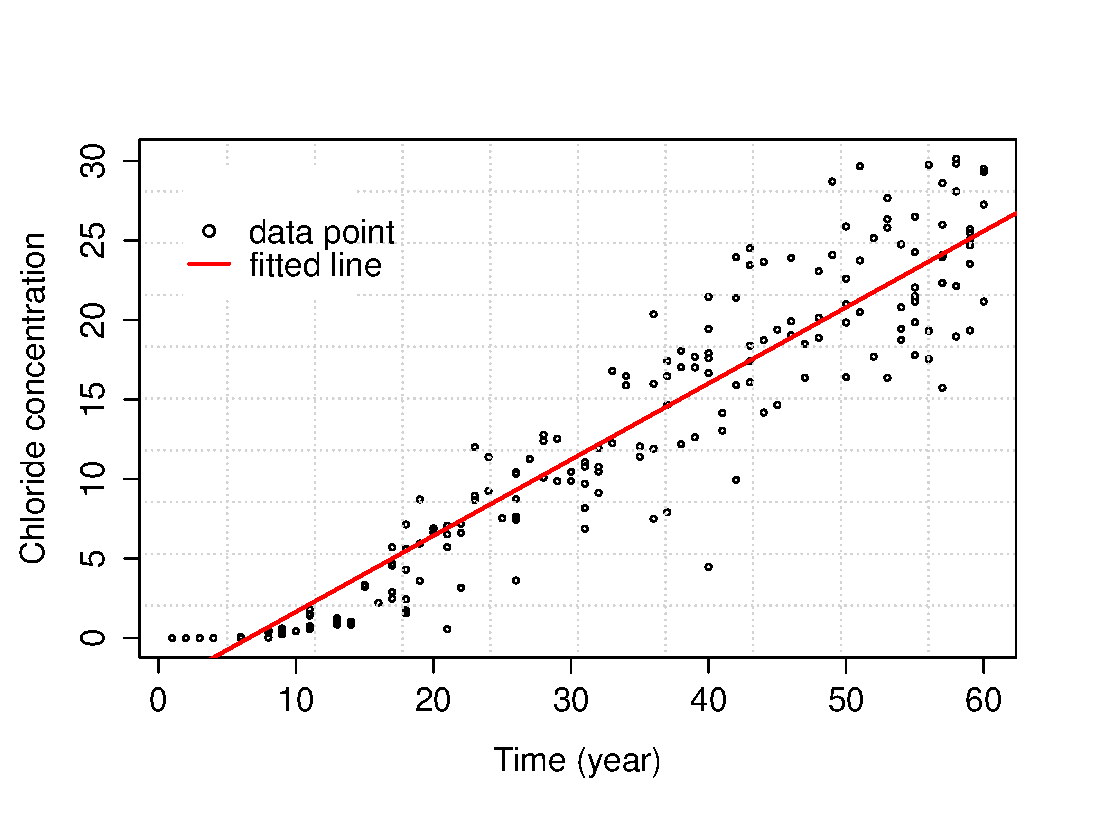
\includegraphics[width=304pt]{fig310.eps}
\caption{Development of chloride concentration}\label{fig:310}
% \end{center}
\end{figure}
The equation to be used for estimating the chloride concentration over time is then

\begin{eqnarray}
 && Y_i^{cl} =  - 3.40275 + 0.47975 \cdot X_i^{cl} \label{eq3225}
\end{eqnarray}
Noted that the value of chloride concentration cannot be negative, therefore, it is necessary to consider a dummy variable to control the results of calculation
\begin{eqnarray}
 && Y_i^{cl} = ( - 3.40275 + 0.47975 \cdot X_i^{cl}) \cdot \delta _i^{cl} \label{eq3226}\\
 && where{\rm{\hspace{2mm} }}\delta _i^{cl} = \left\{ {\begin{array}{*{20}{c}}
{0{\rm{\hspace{2mm}   when \hspace{2mm} X}}_i^{cl} < 7}\\
{1{\rm{\hspace{2mm}   when \hspace{2mm}  X}}_i^{cl} \ge 7{\rm{ }}}
\end{array}} \right.
\end{eqnarray}
Where 7 is the integer value closest to the ratio 3.40275/0.4975. An integer value is used here as the years are used as discrete units of time. 

This result is obtained by running the R code provided in the Appendix \ref{mepi3} on data created using the Appendix \ref{mepi2}.
%
\paragraph{Deterioration: Crack propagation}
To estimate the development of crack width using a regression model, a step similar to the one in section \ref{chrloride} is used. Following results (listing \ref{mechaempicrack}) are obtained (using the R code provided in the Appendix \ref{mepi3}).

\lstinputlisting[basicstyle=\ttfamily\scriptsize,float=h,frame=tb,caption=Results-Crack,label=mechaempicrack]{./Programs/IMP-mecha-empi/IMP-crackpropa.tex}

\begin{figure}[h]
% \begin{center}
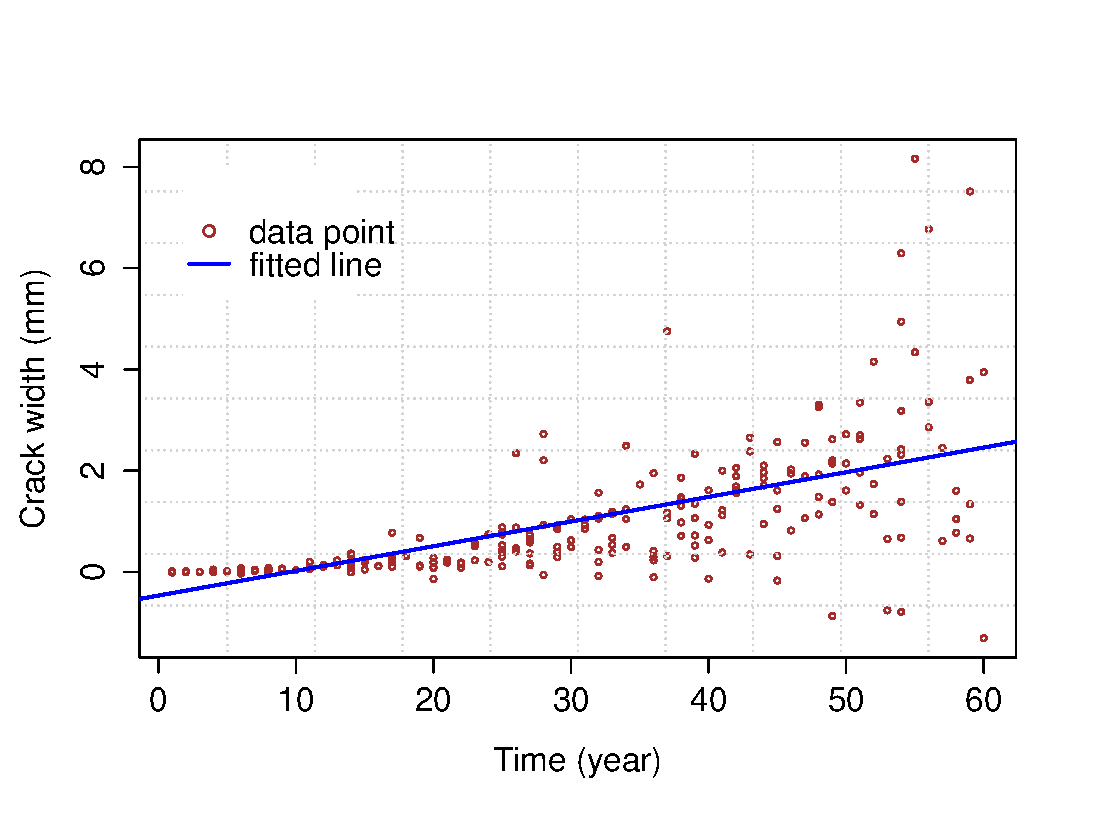
\includegraphics[width=305pt]{fig311.eps}
\caption{Development of crack width}
\label{fig:311}
% \end{center}
\end{figure}
The equation to be used to predict crack width is then:
\begin{eqnarray}
 && Y_i^{cr} = ( - 0.500755 + 0.053150 \cdot X_i^{cr}) \cdot \delta _i^{cr} \label{eq3227}\\
 && where{\rm{\hspace{2mm} }}\delta _i^{cr} = \left\{ {\begin{array}{*{20}{c}}
{0{\rm{ \hspace{2mm}  when \hspace{2mm} X}}_i^{cr} < 9}\\
{1{\rm{ \hspace{2mm}  when \hspace{2mm}  X}}_i^{cr} \ge 9{\rm{ }}}
\end{array}} \right.
\end{eqnarray}
Where 9 is the integer value closest to the ratio 0.500755/0.053150. An integer value is used here as the years are used as discrete units of time.
%
\paragraph{Deterioration prediction}

Using the regression equations given above, the predicted deterioration is as shown in Figure \ref{fig:312}. The curve consists of three pieces. The first piece represents the period of time from new construction until the chloride concentration at the reinforcement level is thought to be equivalent to that determined by the regression equation. The second piece represents the period of time where the chloride concentration at the reinforcement can be represented by the regression equation to the point where corrosion has started to an extent to cause at least one crack wider than 0.5 mm, and the third piece shows the propagation phase, i.e. the extension of cracking once at least one crack is wider than 0.5 mm. This is represented by the second regression equation.
\begin{figure}[h]
% \begin{center}
\includegraphics[width=305pt]{fig312.eps}
\caption{Development of crack width}
 \label{fig:312}
% \end{center}
\end{figure}
\paragraph{Results}
As can be seen from the deterioration curve estimated by using regression model, by the time of 17 years, the chloride concentration certainly reach to a level that higher than 0.48. It means the bridge slab will enter CS 3 and the second phase of deterioration will start, which initiates cracking. Since the time to the worst condition state (CS 5) from the time propagation phase starts will be about 10 years, meaning that the total duration of deterioration from CS1 to CS 5 is about 27 years.

So, since I know that the chloride concentration ${C_{crit}}$ that starts the propagation phase is ${C_{cl}} = {C_{crit}} = 0.48$, and if I consider that once a crack width is 0.5 mm that an intervention is required to ensure that an adequate LOS is provided, I will plan an intervention before year 27. 
\section{Comparison mechanistic-empirical models vs. regression models}
Using both models, and planning an intervention when there is a 50\% chance that the bridge slab will be in CS5 are the same (27 years). 

Using the mechanistic model, in the way we did we could also determine the probability of the bridge slab being in CS5 in each time interval through-out the investigated time period. This made it possible to set other criteria on when to intervene, e.g. the probability of being in CS5 is negligible, or less than 20\%. This was not possible using the regression model the way we did. If it was desired to take into consideration risk, using the regression analysis one would need to arbitrarily pick an earlier point in time to plan the intervention, e.g. in year 20 and not in year 25. 

The use of the mechanistic-empirical model requires a lot of information on the specific values of the parameters to be used in the model, estimates of the uncertainty of the model, and the model. It is suitable in situations where there is not a lot of data on the performance of the deck slabs, and it is feasible to estimate the distributions to be used to represent the values of the parameters, develop the model, and estimate model uncertainty.

The use of the regression model requires a lot of information on the performance of similar deck slabs. It is suitable in situations where this information exists.
\section{Assignments}
\subsection{Problem A - Erosion of concrete cover of waste water tanks}
In a waste water treatment plant, reinforced concrete tanks are used to store the waste water before going through the cleaning process. Waste water is stored in the tanks and various chemical substances are poured into the tanks for the purposes of disinfection. The cement deteriorates due to this exposure. 

The infrastructure manager is interested in predicting the condition of the tanks so that the maintenance interventions can be better planned over the next 30 years. She realizes that these can be estimated using the results of past inspections performed at 2 years intervals (Table \ref{tbl:35}). The first inspection time was executed 1 year after the begin use of the tanks. It is a general rule of thumb that the erosion should not be more than 12 mm.
%
\begin{table}
%	\centering
	\caption{Inspection data} \label{tbl:35}
\begin{tabular}{|l|l|l|l|l|l|}
\hline
\multicolumn{1}{|c|}{Tank} & \multicolumn{5}{c|}{Depth of erosion (m)} \\ 
\cline{2-6}
\multicolumn{1}{|c|}{} & \multicolumn{1}{c|}{inspection 1} & \multicolumn{1}{c|}{inspection 2} & \multicolumn{1}{c|}{inspection 3} & \multicolumn{1}{c|}{inspection 4} & \multicolumn{1}{c|}{inspection 5} \\ 
\hline
\multicolumn{1}{|c|}{1} & \multicolumn{1}{c|}{0.2} & \multicolumn{1}{c|}{1.1} & \multicolumn{1}{c|}{2.4} & \multicolumn{1}{c|}{3.8} & \multicolumn{1}{c|}{4.9} \\ 
\hline
\multicolumn{1}{|c|}{2} & \multicolumn{1}{c|}{0.5} & \multicolumn{1}{c|}{0.9} & \multicolumn{1}{c|}{1.7} & \multicolumn{1}{c|}{3.5} & \multicolumn{1}{c|}{5.2} \\ 
\hline
\multicolumn{1}{|c|}{3} & \multicolumn{1}{c|}{2} & \multicolumn{1}{c|}{2.7} & \multicolumn{1}{c|}{3.2} & \multicolumn{1}{c|}{4.5} & \multicolumn{1}{c|}{5.5} \\ 
\hline
\multicolumn{1}{|c|}{4} & \multicolumn{1}{c|}{1.5} & \multicolumn{1}{c|}{3.1} & \multicolumn{1}{c|}{3.6} & \multicolumn{1}{c|}{5.5} & \multicolumn{1}{c|}{6.3} \\ 
\hline
\multicolumn{1}{|c|}{5} & \multicolumn{1}{c|}{1.1} & \multicolumn{1}{c|}{1.8} & \multicolumn{1}{c|}{1.9} & \multicolumn{1}{c|}{3.1} & \multicolumn{1}{c|}{4.9} \\ 
\hline
\multicolumn{1}{|c|}{6} & \multicolumn{1}{c|}{0.7} & \multicolumn{1}{c|}{1.5} & \multicolumn{1}{c|}{2} & \multicolumn{1}{c|}{3.8} & \multicolumn{1}{c|}{5.1} \\ 
\hline
\multicolumn{1}{|c|}{7} & \multicolumn{1}{c|}{0.8} & \multicolumn{1}{c|}{0.9} & \multicolumn{1}{c|}{1.8} & \multicolumn{1}{c|}{4.2} & \multicolumn{1}{c|}{5.4} \\ 
\hline
\multicolumn{1}{|c|}{8} & \multicolumn{1}{c|}{1} & \multicolumn{1}{c|}{1.9} & \multicolumn{1}{c|}{2.6} & \multicolumn{1}{c|}{3.9} & \multicolumn{1}{c|}{5} \\ 
\hline
\multicolumn{1}{|c|}{9} & \multicolumn{1}{c|}{0.9} & \multicolumn{1}{c|}{1.7} & \multicolumn{1}{c|}{3.6} & \multicolumn{1}{c|}{4.3} & \multicolumn{1}{c|}{7.1} \\ 
\hline
\multicolumn{1}{|c|}{10} & \multicolumn{1}{c|}{0.8} & \multicolumn{1}{c|}{0.9} & \multicolumn{1}{c|}{1.6} & \multicolumn{1}{c|}{4.1} & \multicolumn{1}{c|}{6.7} \\ 
\hline
\multicolumn{1}{|c|}{11} & \multicolumn{1}{c|}{0.5} & \multicolumn{1}{c|}{1.8} & \multicolumn{1}{c|}{2.3} & \multicolumn{1}{c|}{3.7} & \multicolumn{1}{c|}{5.8} \\ 
\hline
\multicolumn{1}{|c|}{12} & \multicolumn{1}{c|}{0.6} & \multicolumn{1}{c|}{1.2} & \multicolumn{1}{c|}{2.2} & \multicolumn{1}{c|}{3.6} & \multicolumn{1}{c|}{6} \\ 
\hline
\end{tabular}
\end{table}

She also realizes that this can be done using by constructing and testing tank walls in the laboratory. After having done this her engineers have come up with the following mechanistic deterioration model.
\begin{eqnarray}
 && f(t + 1) = f(t) \cdot {e^\beta }\label{eq3228}
\end{eqnarray}
Where:
\begin{adjustwidth}{1cm}{}
\begin{description}
\item[$f(t+1)$:] is the depth of corrosion.
\item[$\beta$:] is the deterioration coefficient taking its value of 0.1.
\end{description}
%\end{flushright}
\end{adjustwidth}
It is assumed that $f(0) = 0$ and $f(1) = 1$\footnote{This assumption is used to prevent the value of function $f$ to be equal to 0 at year t=0}.

\subsection{Question A1}
What is the condition of each object in 30 years if the mechanistic-empirical model is used?
\subsection{Question A2}
What is the condition of each object in 30 years if predictions are made using a regression analysis?
\subsection{Answer A1}
Using Eq. \eqref{eq3228}, the evolution of erosion over 30 years is shown in Table \ref{tbl:36} and Figure \ref{fig:313}. 

\begin{table}
%	\centering
	\caption{Evolution of erosion (mechanistic-empirical model)} \label{tbl:36}
\begin{tabular}{|l|l|l|l|l|l|}
\hline
\multicolumn{1}{|c|}{Time} & \multicolumn{1}{c|}{Erosion} & \multicolumn{1}{c|}{Time} & \multicolumn{1}{c|}{Erosion} & \multicolumn{1}{c|}{Time} & \multicolumn{1}{c|}{Erosion} \\ 
\multicolumn{1}{|c|}{(years)} & \multicolumn{1}{c|}{(mm)} & \multicolumn{1}{c|}{(years)} & \multicolumn{1}{c|}{(mm)} & \multicolumn{1}{c|}{(years)} & \multicolumn{1}{c|}{(mm)} \\ 
\hline
\multicolumn{1}{|c|}{1} & \multicolumn{1}{c|}{1} & \multicolumn{1}{c|}{11} & \multicolumn{1}{c|}{2.7183} & \multicolumn{1}{c|}{21} & \multicolumn{1}{c|}{7.3891} \\ 
\hline
\multicolumn{1}{|c|}{2} & \multicolumn{1}{c|}{1.1052} & \multicolumn{1}{c|}{12} & \multicolumn{1}{c|}{3.0042} & \multicolumn{1}{c|}{22} & \multicolumn{1}{c|}{8.1662} \\ 
\hline
\multicolumn{1}{|c|}{3} & \multicolumn{1}{c|}{1.2214} & \multicolumn{1}{c|}{13} & \multicolumn{1}{c|}{3.3201} & \multicolumn{1}{c|}{23} & \multicolumn{1}{c|}{9.0250} \\ 
\hline
\multicolumn{1}{|c|}{4} & \multicolumn{1}{c|}{1.3499} & \multicolumn{1}{c|}{14} & \multicolumn{1}{c|}{3.6693} & \multicolumn{1}{c|}{24} & \multicolumn{1}{c|}{9.9742} \\ 
\hline
\multicolumn{1}{|c|}{5} & \multicolumn{1}{c|}{1.4918} & \multicolumn{1}{c|}{15} & \multicolumn{1}{c|}{4.0552} & \multicolumn{1}{c|}{25} & \multicolumn{1}{c|}{11.0232} \\ 
\hline
\multicolumn{1}{|c|}{6} & \multicolumn{1}{c|}{1.6487} & \multicolumn{1}{c|}{16} & \multicolumn{1}{c|}{4.4817} & \multicolumn{1}{c|}{26} & \multicolumn{1}{c|}{12.1825} \\ 
\hline
\multicolumn{1}{|c|}{7} & \multicolumn{1}{c|}{1.8221} & \multicolumn{1}{c|}{17} & \multicolumn{1}{c|}{4.9530} & \multicolumn{1}{c|}{27} & \multicolumn{1}{c|}{13.4637} \\ 
\hline
\multicolumn{1}{|c|}{8} & \multicolumn{1}{c|}{2.0138} & \multicolumn{1}{c|}{18} & \multicolumn{1}{c|}{5.4739} & \multicolumn{1}{c|}{28} & \multicolumn{1}{c|}{14.8797} \\ 
\hline
\multicolumn{1}{|c|}{9} & \multicolumn{1}{c|}{2.2255} & \multicolumn{1}{c|}{19} & \multicolumn{1}{c|}{6.0496} & \multicolumn{1}{c|}{29} & \multicolumn{1}{c|}{16.4446} \\ 
\hline
\multicolumn{1}{|c|}{10} & \multicolumn{1}{c|}{2.4596} & \multicolumn{1}{c|}{20} & \multicolumn{1}{c|}{6.6859} & \multicolumn{1}{c|}{30} & \multicolumn{1}{c|}{18.1741} \\ 
\hline
\end{tabular}
\end{table}

\begin{figure}[h]
% \begin{center}
\includegraphics[width=300pt]{fig313.eps}
\caption{Evolution of erosion – mechanistic-empirical model}
 \label{fig:313}
% \end{center}
\end{figure}
%
By the year 26, if the infrastructure manager has not already executed an intervention, the depth of erosion will reach 12 mm, which is beyond the critical level. In order to prevent the re-bars of tanks from the onset of corrosion, an intervention (e.g. renewal of cover layer of the tanks walls) should be executed before year 26. 
\subsection{Answer A2}
Assuming that the form of the regression is linear, the general regression equation is:
\begin{eqnarray}
 && Y_i^{ero} = {\alpha _{ero}} + {\beta _{ero}} \cdot X_i^{ero} + \varepsilon _i^{ero} \label{eq3229}
\end{eqnarray}
Where:
\begin{adjustwidth}{1cm}{}
\begin{description}
\item[$Y_i^{ero}$:] is the value of erosion at year \textit{i}.
\item[$X_i^{ero}$:] is the year \textit{i}.
\item[${\alpha _{ero}},{\beta _{ero}}$:] are regression parameters that need to be estimated.
\item[$\varepsilon _i^{ero}$:] is the prediction errors following a normal distribution
\end{description}
%\end{flushright}
\end{adjustwidth}
Using the linear regression analysis (refer to section \ref{regressionmodel}), and in the Appendix \ref{mepi4}, following results are obtained (listing \ref{mechaempiwaste}).

\lstinputlisting[basicstyle=\ttfamily\scriptsize,float=h,frame=tb,caption=Results,label=mechaempiwaste]{./Programs/IMP-mecha-empi/IMP-A-waste-water-tanks.tex}

\begin{eqnarray}
 && Y_i^{ero} =  - 0.03630 + 0.59171 \cdot X_i^{ero} \label{eq3230}
\end{eqnarray}
\begin{figure}[h]
% \begin{center}
\includegraphics[width=302pt]{fig314.eps}
\caption{Evolution of erosion - linear regression model}\label{fig:314}
% \end{center}
\end{figure}
 
The fitted line plotted from Eq. \eqref{eq3230} is shown in Figure \ref{fig:314}. When the level of erosion becomes 12 mm, it corresponds to 20 years. If the infrastructure manager relies solely on this analysis she will plan the intervention to be executed before year 20.
\subsection{Problem B - Bridge wear out}
An infrastructure manager wants to make a work program for a bridge, i.e. when an intervention needs to be executed and what type of intervention. He normally models deterioration using the following mechanistic-empirical model:
\begin{eqnarray}
 && I = \exp (\lambda  \cdot t) - 1 \label{eq3231}
\end{eqnarray}
Where is $\lambda $is the deterioration coefficient, which is given by:
\begin{eqnarray}
 && \lambda  = \frac{{\ln (2)}}{{Tc}} \label{eq3232}
\end{eqnarray}
In Eq. \eqref{eq3231}, $Tc$ represents the average life time of the structure elements of the bridge. It is modeled using a normal distribution with mean and standard deviation equal to 60 years and 7 years, respectively. A detail description of the model can be referred to the work of \cite{Brodsky2006}. The manager divides condition into five discrete states given in Table \ref{tbl:37}. The wear out of the bridge has its value from 0 to 1 as defined in Eq. \eqref{eq3232}.
\begin{table}
%	\centering
	\caption{Definition of condition states} \label{tbl:37}
\begin{tabular}{|l|l|l|}
\hline
\multicolumn{1}{|c|}{Condition states} & \multicolumn{1}{c|}{Description} & \multicolumn{1}{c|}{Corresponding values of I} \\ 
\hline
\multicolumn{1}{|c|}{1} & \multicolumn{1}{c|}{New/Partially new} & \multicolumn{1}{c|}{$I<0.2$} \\ 
\hline
\multicolumn{1}{|c|}{2} & \multicolumn{1}{c|}{Good} & \multicolumn{1}{c|}{$0.2\le I <0.4$} \\ 
\hline
\multicolumn{1}{|c|}{3} & \multicolumn{1}{c|}{Average} & \multicolumn{1}{c|}{$0.4\le I <0.6$} \\ 
\hline
\multicolumn{1}{|c|}{4} & \multicolumn{1}{c|}{Bad} & \multicolumn{1}{c|}{$0.6\le I <0.8$} \\ 
\hline
\multicolumn{1}{|c|}{5} & \multicolumn{1}{c|}{Very bad} & \multicolumn{1}{c|}{$I\ge0.8$}\\
\hline
\end{tabular}
\end{table}
\subsection{Question}
What is the probabilistic distribution of discrete condition states over the next 50 years for the bridge? What does this mean?

\subsection{Answer}
As the value of $Tc$ is probabilistic in nature, the value of I is also probabilistic. A Monte Carlo simulation with 20'000 iterations is used to estimate the probability of \textit{I} having values that correspond with each of the condition states over time. The results are shown in Figure \ref{fig:315}. The R code in the Appendix \ref{mepi5} is used to estimate the probability of the bridge being in each condition state over 50 years. 
\begin{figure}[h]
% \begin{center}
\includegraphics[width=300pt]{fig315.eps}
\caption{Condition state distribution over 50 years}\label{fig:315}
% \end{center}
\end{figure}
As can be seen from the figure, in the first 10 years after the construction of the bridge, the bridge will remains in CS1. Then, the probability that the bridge is in CS1 decreases and the probability that it will be in CS2 increases. After 30 years, there is a 50\% probability that the bridge will be in CS2.

After 30 years, there is a small probability that the bridge will be in CS3, and after 40 years, a 50\% probability that the bridge will be in CS 4. The speed of degradation increases rapidly after 30 years. By year 50, the probability that the bridge is in CS 5 is more than 50\%. 

Based on this information the infrastructure manager might consider executing an intervention before year 40 to avoid an inadequate LOS from occurring. The steps of numerical calculation can be tracked by reading the R script for this example provided at the the Appendix \ref{mepi5}.

%
\bibliographystyle{plainnat}
\bibliography{reference}
\pagebreak

\begin{subappendices}
% \label{appendix3}
% \label{appendix3}
\section{R code for the mechanistic-empirical model-concrete bridge slab}\label{mepi1}
% \textbf{R code for the mechanistic-empirical model-concrete bridge slab}
\lstinputlisting[basicstyle=\ttfamily\scriptsize]{./Programs/IMP-mecha-empi/IMP-Mechanistic-Emprical-model.r}
\pagebreak
\section{R code for generating data}\label{mepi2}
% \textbf{R code for generating data}
\lstinputlisting[basicstyle=\ttfamily\scriptsize]{./Programs/IMP-mecha-empi/IMP-data-generation.r}
\pagebreak
\section{R code for regression analysis} \label{mepi3}
% \textbf{R code for regression analysis}
\lstinputlisting[basicstyle=\ttfamily\scriptsize]{./Programs/IMP-mecha-empi/IMP-regression.r}
\pagebreak
\section{R code for estimation of erosion evolution over 30 years} \label{mepi4}
% \textbf{R code for estimation of erosion evolution over 30 years}
\lstinputlisting[basicstyle=\ttfamily\scriptsize]{./Programs/IMP-mecha-empi/IMP-A-waste-water-tanks.r}
\pagebreak
\section{R code for chloride concentration} \label{mepi5}
% \textbf{R code for chloride concentration}
\lstinputlisting[basicstyle=\ttfamily\scriptsize]{./Programs/IMP-mecha-empi/IMP-A-bridge-wear-out.r}
\end{subappendices}
% \pagebreak
% \section*{Appendix 3.4} \label{mepi4}
% \textbf{R code for regression analysis}
% \lstinputlisting{./Programs/IMP-chapter3-R/IMP-4-regression.r}

 
 
 
 
 
 
 